%-----------------------------------------------------------------------------------------------
\makeatletter
\immediate\write18{datelog > \jobname.info} % site script for $(date '+%Y-%m-%d %Hh%Mm%Ss')
\makeatother
%-----------------------------------------------------------------------------------------------
\usepackage{beamerthemeCopenhagen}
\usepackage[utf8]{inputenc}
\usepackage[english,brazil]{babel} % last becomes the active one
\usepackage{pslatex}
\usepackage{amssymb,amsmath}
\usepackage{soul}
\usepackage[squaren,Gray]{SIunits}
\usepackage{xspace}
%-----------------------------------------------------------------------------------------------
\definecolor{enfa}{rgb}{0.71,0.69,0.67} % Emphasis
%-----------------------------------------------------------------------------------------------
\newcommand{\enfa}[1]{{\color{enfa}{#1}}}
\newcommand{\gray}[1]{{\color{gray}{#1}}}
\newcommand{\txtpic}[1]{%
    \fcolorbox{lightgray}{white!90!black}{{#1}} 
}
%-----------------------------------------------------------------------------------------------
\newcommand{\vet}[1]{\underline{{#1}}}
\newcommand{\mat}[1]{\underline{\underline{{#1}}}}
\newcommand{\cub}[1]{\underline{\underline{\underline{{#1}}}}}
\newcommand{\eqdef}{{\ensuremath\stackrel{\text{\tiny def}}{=}}}
%-----------------------------------------------------------------------------------------------
\title{A.03.01 -- Sistemas Fechados}
\subtitle{Trabalho de Fronteira}
\author{Prof.~C.~Naaktgeboren}
\date{\tt Compiled on \input{\jobname.info}}
%-----------------------------------------------------------------------------------------------
\begin{document}
%-----------------------------------------------------------------------------------------------
\logo{
\includegraphics[height=0.8cm]{root/00-res/logo/CNThermSci-logo-A.pdf}} % Alpha logo
%-----------------------------------------------------------------------------------------------
%{%
%    \usebackgroundtemplate{%
%        \parbox{\paperwidth}{%
%            \vspace*{1sp}\centering\includegraphics[height=\paperheight]%
%                {art/landscape-615428_1280.jpg}
%    }}
    \frame{\titlepage}
%}
%-----------------------------------------------------------------------------------------------
%{%
%    \usebackgroundtemplate{%
%         \parbox{\paperwidth}{%
%             \vspace*{1sp}\centering\includegraphics[height=\paperheight]%
%                 {art/mountains-landscape-1149580_1280.jpg}
%    }}
%    \frame{\tableofcontents}
%}
%-----------------------------------------------------------------------------------------------
\section{Trabalho de Fronteira}

    % !j 96 -i8
    %-------------------------------------------------------------------------------------------
    \frame{
        \frametitle{Trabalho de Fronteira}\vspace*{-2em}

        Trabalho de fronteira, $W_f$  (\kilo\joule),  é  a  \enfa{interação  energética}  de  um
        sistema  compressível  simples  capaz  de  \enfa{diretamente}  realizar   \enfa{trabalho
        mecânico},   $W_m   \equiv   \vet{F}\cdot\vet{\ell}$   (\kilo\joule),   por   meio    do
        \enfa{deslocamento} de uma \enfa{fronteira móvel}:

        \begin{figure}
            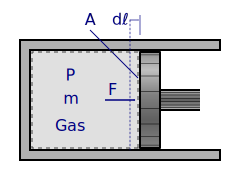
\includegraphics[width=5.0cm]{fig/A0301-pt-01-HPistCyl.pdf}
        \end{figure}
    }
    %-------------------------------------------------------------------------------------------

    % !j 96 -i8
    %-------------------------------------------------------------------------------------------
    \frame{
        \frametitle{Trabalho de Fronteira}\vspace*{-2em}

        Trabalho de fronteira, $W_f$  (\kilo\joule),  é  a  \enfa{interação  energética}  de  um
        sistema  compressível  simples  capaz  de  \enfa{diretamente}  realizar   \enfa{trabalho
        mecânico},   $W_m   \equiv   \vet{F}\cdot\vet{\ell}$   (\kilo\joule),   por   meio    do
        \enfa{deslocamento} de uma \enfa{fronteira móvel}:

        \begin{figure}
            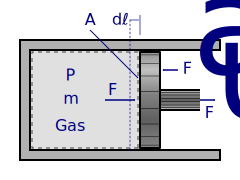
\includegraphics[width=5.0cm]{fig/A0301-pt-02-HPistCyl.pdf}
        \end{figure}
    }
    %-------------------------------------------------------------------------------------------

    % !j 96 -i8
    %-------------------------------------------------------------------------------------------
    \frame{
        \frametitle{Trabalho de Fronteira}\vspace*{-2em}

        \begin{figure}
            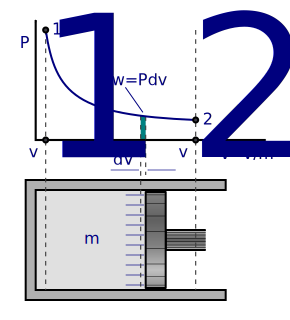
\includegraphics[width=5.0cm]{fig/A0301-pt-03-HPistCylPlot.pdf}
        \end{figure}

    }
    %-------------------------------------------------------------------------------------------

\section{Tópicos de Leitura}

    %------------------------------------------------------------------------------------------
    \frame{
        \frametitle{Tópicos de Leitura}\vspace*{-2em}

        \begin{thebibliography}{Çengel, Y.~A., 2013}

            \bibitem[Çengel, Y.~A., 2013]{2013-CengelYA+BolesMA-AMGH}
                Çengel, Y.~A. e Boles, M.~A.
                \newblock{{\em Termodinâmica $7^\mathrm{a}\!$ Ed.} \enfa{Sec.~4--1}.}
                \newblock{AMGH. Porto Alegre. 978-85-8055-200-3.}

        \end{thebibliography}
    }
    %------------------------------------------------------------------------------------------

%-----------------------------------------------------------------------------------------------
\end{document}
%-----------------------------------------------------------------------------------------------

